\subsection{Test 3:}

The third test consists to prove that the {\bfseries Hamiltonian-Cycle} in Figure 4.3.0 is actually one ( {\itshape C = [ 1, 2, 3, 4, 5, 6, 7, 8, 1 ]} ). Once we have declared the graph and the certificate, we run the program and see the console output ( Figure 4.3.1 ) and the plot of the computational time of the algorithm ( Figure 4.3.2 ). Finally the table 3 describe the point of Figure 4.3.2. \hfill \break

\begin{figure}[H]
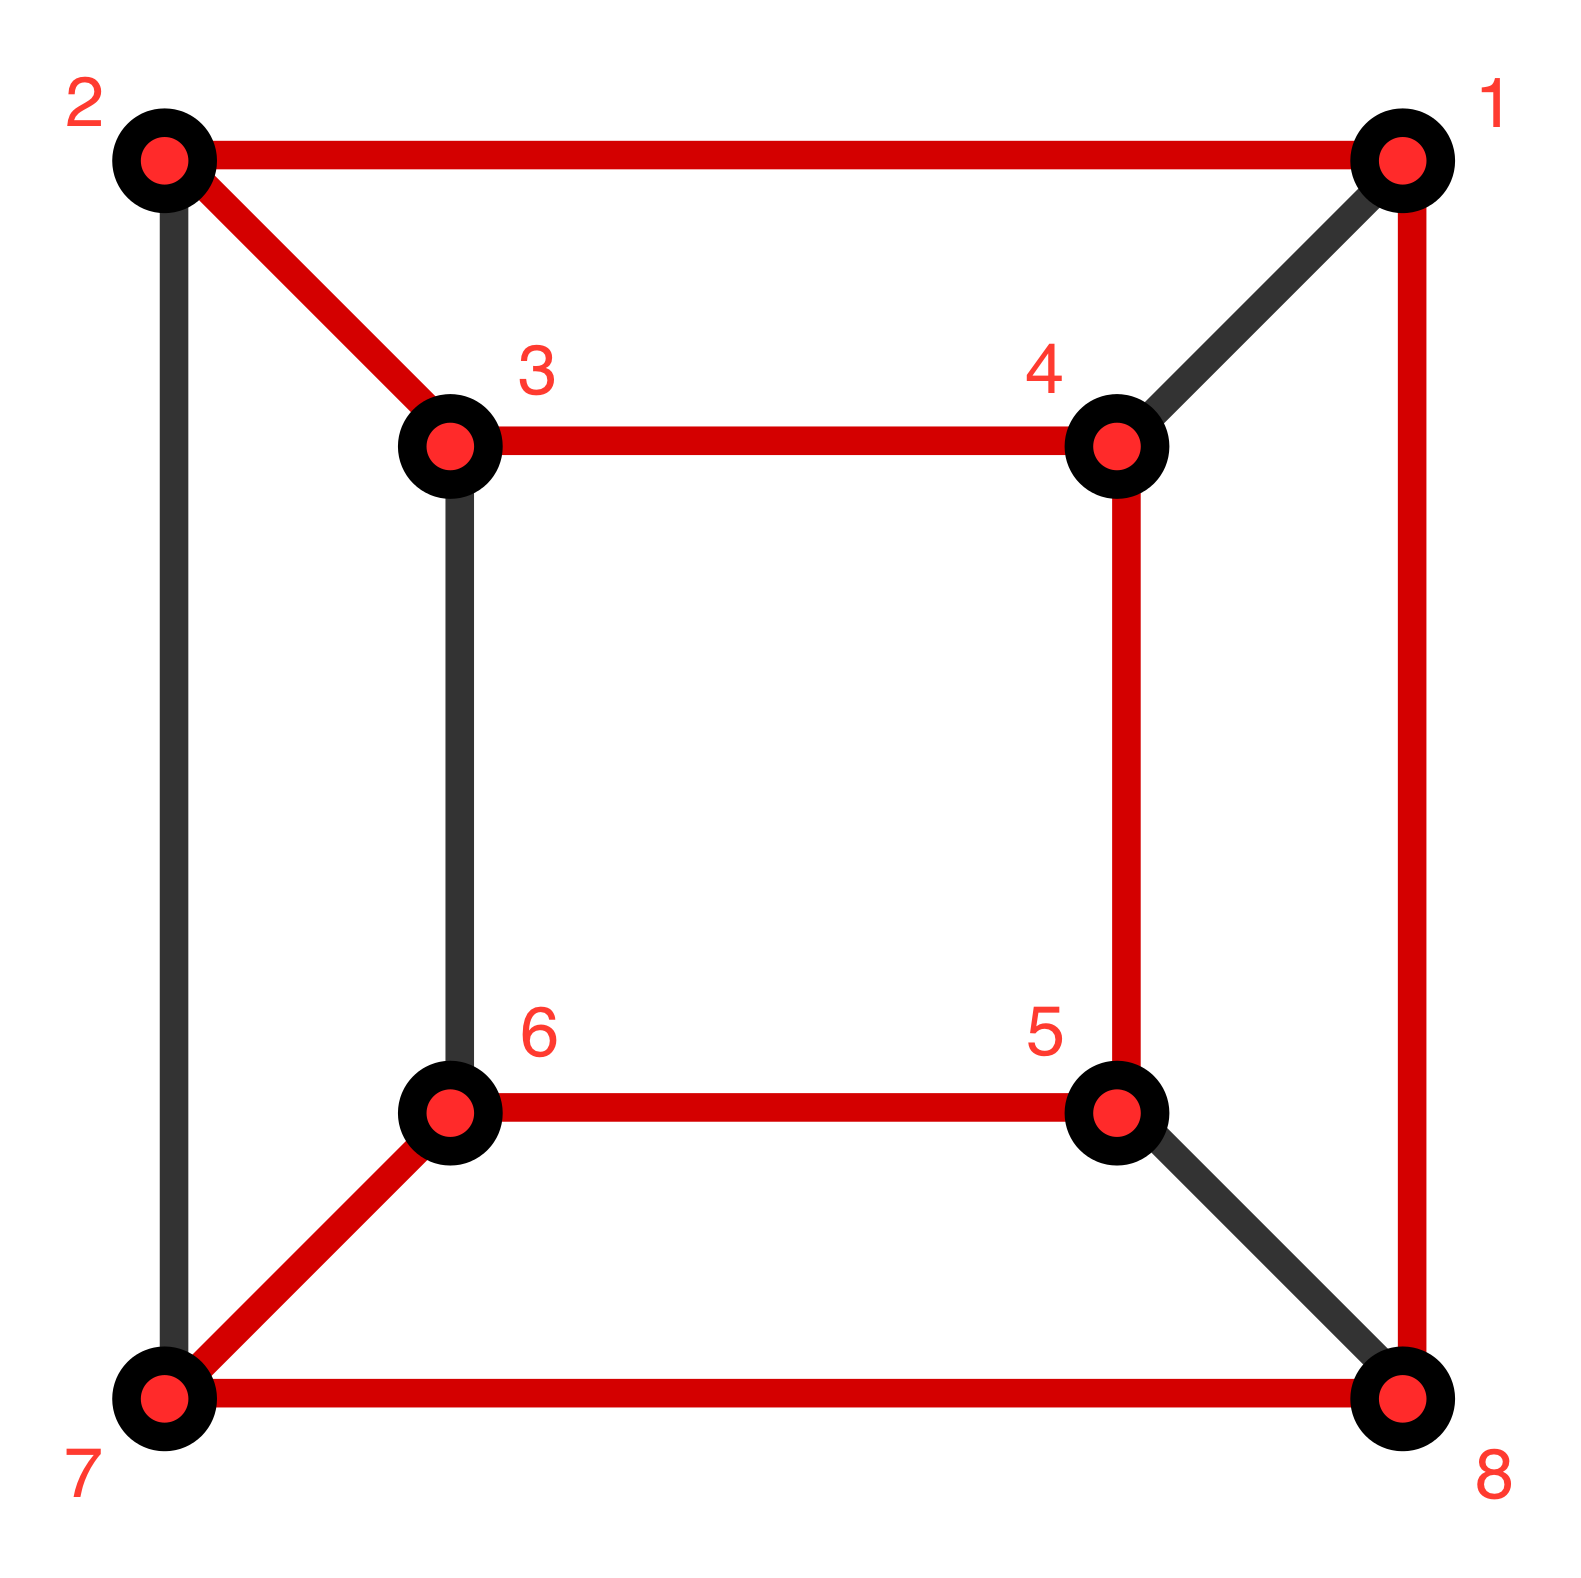
\includegraphics[height = 6cm, width = 8cm]{12.png}
\centering \linebreak \linebreak {\small Figure 4.3.0: Graph to analyze.}
\end{figure} \hfill \break

\begin{lstlisting}
def main ( ):
    graph = { 1: [ 2, 4, 8 ], 2: [ 7, 3, 1 ], 3: [ 2, 6, 4 ],
              4: [ 1, 3, 5 ], 5: [ 4, 8, 6 ], 6: [ 5, 3, 7 ],
              7: [ 6, 2, 8 ], 8: [ 7, 5, 1 ] }
    certificate = [ 1, 2, 3, 4, 5, 6, 7, 8, 1 ]
    verify_hamiltonian ( graph, certificate )
\end{lstlisting} \hfill \break

\begin{figure}[H]
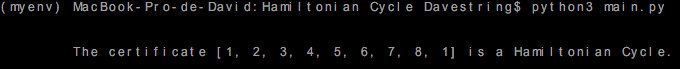
\includegraphics[height = 1.5cm, width = 16.5cm]{12c.png}
\centering \linebreak \linebreak {\small Figure 4.3.1: Console output.}
\end{figure} \hfill \break

\begin{center}
\begin{tabular}{c c}
\toprule \toprule
\hspace{100px} Graph Size \hspace{90px} & \hspace{100px} Time \hspace{90px} \\
\midrule \midrule
0 & 4 \\
\midrule
1 & 7 \\
\midrule
2 & 10 \\
\midrule
3 & 12 \\
\midrule
4 & 14 \\
\midrule
5 & 16 \\
\midrule
6 & 18 \\
\midrule
7 & 20 \\
\bottomrule
\end{tabular}
\centering \linebreak \linebreak Table 3.
\end{center}

\begin{figure}[H]
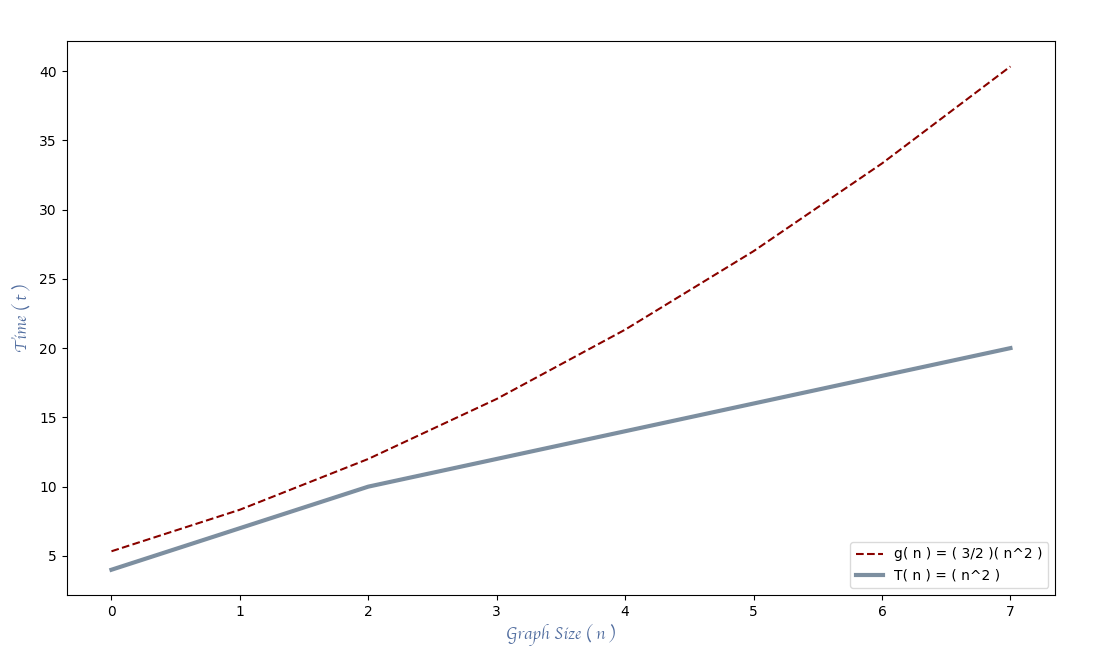
\includegraphics[height = 8cm, width = 16.5cm]{12g.png}
\centering \linebreak \linebreak {\small Figure 4.3.2: Plot of the algorithm.}
\end{figure} \hfill \break